\section{Архитектура}
\label{sec:Arch}

Семейство видеокарт Intel $X^e$ состоит из различных микроархитектур, включающих энергоэффективные модели $X^e$-LP и высокопроизводительных $X^e$-HPG и $X^e$-HPC~\cite{intelArch}, ориентированных на игры и вычисления.

Для LP одновременно выполняемые потоки (SMT) объединены в Execution Unit (EU).
Каждый EU состоит из семи потоков SMT. Главный вычислительный модуль состоит из SIMD8 ALU, поддерживающий SIMD8 FP/INT операции -- целочисленные или с плавающей точкой, и SIMD2 ALU, поддерживающий расширенные математические операции.
Каждый поток имеет 128 регистров (general-purpose registers) каждый размером 32 байта.
Вся совокупность регистров для одного потока называется general register file (GRF).
Важной концепцией является Shared Local Memory (SLM) -- это общая память на рабочую группу потоков.
16 EUs объединены в Dual Subslice (DSS) с кэшем инструкций, памятью SLM и портом 128B/cycle.
Два EU могут быть объединены в пару для выполнения SIMD16 инструкций. Каждые 6 DSS объединены в Slice вместе с 16MB L3 кэшем.

В отличие от LP, где в качестве вычислительной ячейки используется EU, в HPC и HPG используются $X^e$-core, похожие на LP DSS.
$X^e$-core содержит 8 векторных и 8 матричных движков, которые производят высокопроизводительные вычисления.
Core объединены в Slice, Slice в Stack.
В итоге получается объединение большого числа вычислительных потоков.

Все вычисления выполняются над данными, расположенными в регистрах -- сверхбыстрая память, располагающаяся непосредственно рядом с вычислительными элементами.
Преимущество в скорости накладывает сильное ограничение на размер регистровой памяти.
Чтобы эффективно расположить данные на регистрах используется алгоритм раскрашивания RIG (Register interference graph)~\cite{regalloc}.

Наибольший вред производительности наносит выход за пределы регистрового файла.
Тогда перед использованием данных они загружаются из памяти (fill), а после использования -- выгружаются обратно (spill).
Поскольку работа с памятью на порядок медленнее работы с регистрами, в важных частях программы возникают задержки, и общая производительность снижается катастрофически.

Скорость обращения к данным для видеускорителей так же сильно отличается в зависимости от используемой памяти.
К данным на регистрах обращение идёт напрямую, в то время как обращение к данным в TPM (Thread Private Memory -- индивидуальное место в памяти для потока) идёт опосредованно, с предварительной загрузкой/отправкой этих данных сообщением send.
Схематичное изображение регистрового файла и TPM на Рис~\ref{fig:mem}.
Для видеускорителей критически необходим быстрый доступ к данным, иначе потоки будут большую часть времени проводить в ожидании.
Поэтому нужно данные с наиболее частым обращением раскладывать на регистры. Регистров в GPU больше чем в CPU, и они представляют собой регистровую матрицу.

\begin{figure}[ht]
    \centering
    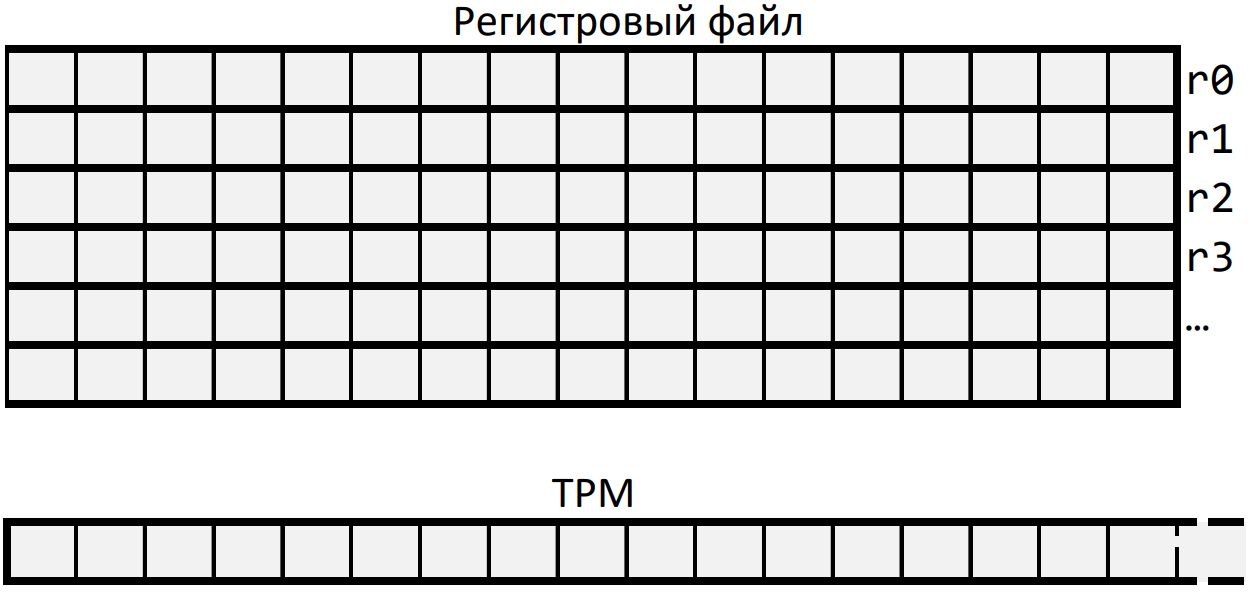
\includegraphics[scale=0.17]{Images/grf_empty.png}
    \caption{Репрезентация регистрового файла и TPM.}
    \label{fig:mem}
\end{figure}

Векторный компилятор Intel имеет возможность векторизовать и разложить на регистры последовательные типы данных. В них входят вектора, массивы, структуры, состоящие из элементов одного примитивного типа и так далее.
Так, например, компилятор может обработать структуру \verb|type {float, <7 x float>}| и преобразовать её в вектор \verb|<8 x float>|.

\begin{figure}[ht]
    \centering
    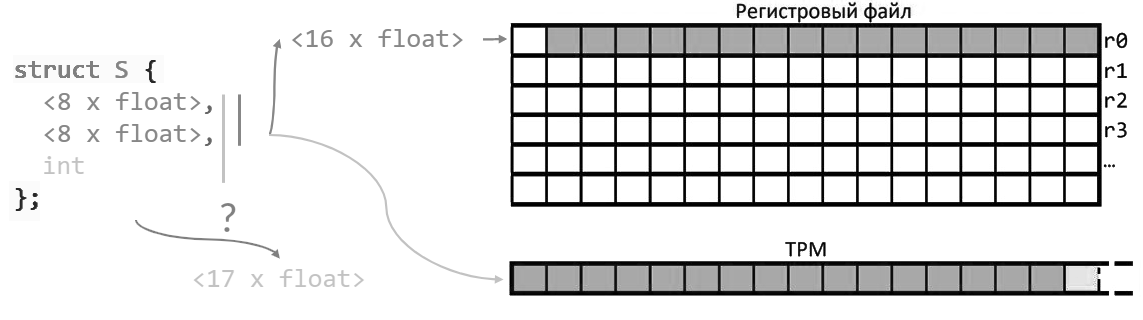
\includegraphics[scale=0.22]{Images/struct_gray.png}
    \caption{Возможное расположение структуры в памяти.}
    \label{fig:lying}
\end{figure}

Однако, векторизация не справляется с более сложными структурами. На рис.~\ref{fig:lying} видно, что структура S без поля int может быть оптимизирована, векторизована и положена на регистры.
Но как только появляется дополнительное поле иного типа, в данном случае это int, встаёт вопрос как векторизовать такой объединённый тип.
Это приводит к использованию структур из памяти, появлению spill'ов и, таким образом, к сильному падению производительности.
Обсуждаемое ниже решение проблемы векторизации структур, также решает проблему размещения структур на регистры и сокращает количество обращений в память.
